\documentclass[11pt,preprint, authoryear]{elsarticle}

\usepackage{lmodern}
%%%% My spacing
\usepackage{setspace}
\setstretch{1.5}
\DeclareMathSizes{12}{14}{10}{10}

% Wrap around which gives all figures included the [H] command, or places it "here". This can be tedious to code in Rmarkdown.
\usepackage{float}
\let\origfigure\figure
\let\endorigfigure\endfigure
\renewenvironment{figure}[1][2] {
    \expandafter\origfigure\expandafter[H]
} {
    \endorigfigure
}

\let\origtable\table
\let\endorigtable\endtable
\renewenvironment{table}[1][2] {
    \expandafter\origtable\expandafter[H]
} {
    \endorigtable
}


\usepackage{ifxetex,ifluatex}
\usepackage{fixltx2e} % provides \textsubscript
\ifnum 0\ifxetex 1\fi\ifluatex 1\fi=0 % if pdftex
  \usepackage[T1]{fontenc}
  \usepackage[utf8]{inputenc}
\else % if luatex or xelatex
  \ifxetex
    \usepackage{mathspec}
    \usepackage{xltxtra,xunicode}
  \else
    \usepackage{fontspec}
  \fi
  \defaultfontfeatures{Mapping=tex-text,Scale=MatchLowercase}
  \newcommand{\euro}{€}
\fi

\usepackage{amssymb, amsmath, amsthm, amsfonts}

\def\bibsection{\section*{References}} %%% Make "References" appear before bibliography


\usepackage[round]{natbib}

\usepackage{longtable}
\usepackage[margin=2.3cm,bottom=2cm,top=2.5cm, includefoot]{geometry}
\usepackage{fancyhdr}
\usepackage[bottom, hang, flushmargin]{footmisc}
\usepackage{graphicx}
\numberwithin{equation}{section}
\numberwithin{figure}{section}
\numberwithin{table}{section}
\setlength{\parindent}{0cm}
\setlength{\parskip}{1.3ex plus 0.5ex minus 0.3ex}
\usepackage{textcomp}
\renewcommand{\headrulewidth}{0.2pt}
\renewcommand{\footrulewidth}{0.3pt}

\usepackage{array}
\newcolumntype{x}[1]{>{\centering\arraybackslash\hspace{0pt}}p{#1}}

%%%%  Remove the "preprint submitted to" part. Don't worry about this either, it just looks better without it:
\makeatletter
\def\ps@pprintTitle{%
  \let\@oddhead\@empty
  \let\@evenhead\@empty
  \let\@oddfoot\@empty
  \let\@evenfoot\@oddfoot
}
\makeatother

 \def\tightlist{} % This allows for subbullets!

\usepackage{hyperref}
\hypersetup{breaklinks=true,
            bookmarks=true,
            colorlinks=true,
            citecolor=blue,
            urlcolor=blue,
            linkcolor=blue,
            pdfborder={0 0 0}}


% The following packages allow huxtable to work:
\usepackage{siunitx}
\usepackage{multirow}
\usepackage{hhline}
\usepackage{calc}
\usepackage{tabularx}
\usepackage{booktabs}
\usepackage{caption}


\newenvironment{columns}[1][]{}{}

\newenvironment{column}[1]{\begin{minipage}{#1}\ignorespaces}{%
\end{minipage}
\ifhmode\unskip\fi
\aftergroup\useignorespacesandallpars}

\def\useignorespacesandallpars#1\ignorespaces\fi{%
#1\fi\ignorespacesandallpars}

\makeatletter
\def\ignorespacesandallpars{%
  \@ifnextchar\par
    {\expandafter\ignorespacesandallpars\@gobble}%
    {}%
}
\makeatother

\newlength{\cslhangindent}
\setlength{\cslhangindent}{1.5em}
\newenvironment{CSLReferences}%
  {\setlength{\parindent}{0pt}%
  \everypar{\setlength{\hangindent}{\cslhangindent}}\ignorespaces}%
  {\par}


\urlstyle{same}  % don't use monospace font for urls
\setlength{\parindent}{0pt}
\setlength{\parskip}{6pt plus 2pt minus 1pt}
\setlength{\emergencystretch}{3em}  % prevent overfull lines
\setcounter{secnumdepth}{5}

%%% Use protect on footnotes to avoid problems with footnotes in titles
\let\rmarkdownfootnote\footnote%
\def\footnote{\protect\rmarkdownfootnote}
\IfFileExists{upquote.sty}{\usepackage{upquote}}{}

%%% Include extra packages specified by user

%%% Hard setting column skips for reports - this ensures greater consistency and control over the length settings in the document.
%% page layout
%% paragraphs
\setlength{\baselineskip}{12pt plus 0pt minus 0pt}
\setlength{\parskip}{12pt plus 0pt minus 0pt}
\setlength{\parindent}{0pt plus 0pt minus 0pt}
%% floats
\setlength{\floatsep}{12pt plus 0 pt minus 0pt}
\setlength{\textfloatsep}{20pt plus 0pt minus 0pt}
\setlength{\intextsep}{14pt plus 0pt minus 0pt}
\setlength{\dbltextfloatsep}{20pt plus 0pt minus 0pt}
\setlength{\dblfloatsep}{14pt plus 0pt minus 0pt}
%% maths
\setlength{\abovedisplayskip}{12pt plus 0pt minus 0pt}
\setlength{\belowdisplayskip}{12pt plus 0pt minus 0pt}
%% lists
\setlength{\topsep}{10pt plus 0pt minus 0pt}
\setlength{\partopsep}{3pt plus 0pt minus 0pt}
\setlength{\itemsep}{5pt plus 0pt minus 0pt}
\setlength{\labelsep}{8mm plus 0mm minus 0mm}
\setlength{\parsep}{\the\parskip}
\setlength{\listparindent}{\the\parindent}
%% verbatim
\setlength{\fboxsep}{5pt plus 0pt minus 0pt}



\begin{document}



\begin{frontmatter}  %

\title{Sustainability in the Political Economy}

% Set to FALSE if wanting to remove title (for submission)




\author[Add1]{Harriet Catherine Laing}
\ead{harrietclaing@gmail.com}





\address[Add1]{University of Stellenbosch, South Africa}

\cortext[cor]{Corresponding author: Harriet Catherine Laing}

\begin{abstract}
\small{
Abstract to be written here.
}
\end{abstract}

\vspace{1cm}


\begin{keyword}
\footnotesize{
Environmental policy \sep Political economy \sep Numerical model \\
\vspace{0.3cm}
}
\end{keyword}



\vspace{0.5cm}

\end{frontmatter}



%________________________
% Header and Footers
%%%%%%%%%%%%%%%%%%%%%%%%%%%%%%%%%
\pagestyle{fancy}
\chead{}
\rhead{}
\lfoot{}
\rfoot{\footnotesize Page \thepage}
\lhead{}
%\rfoot{\footnotesize Page \thepage } % "e.g. Page 2"
\cfoot{}

%\setlength\headheight{30pt}
%%%%%%%%%%%%%%%%%%%%%%%%%%%%%%%%%
%________________________

\headsep 35pt % So that header does not go over title




\hypertarget{introduction}{%
\section{\texorpdfstring{Introduction
\label{Introduction}}{Introduction }}\label{introduction}}

(approx. 800)

The primary objective of this research assignment is to model how
interactions in the political economy inhibit the advancement of
environmental policies. Ultimately, we wish to understand how the
frictions and dominance of certain countries in the global area impacts
global environmental policy. For example, the US is a relatively smaller
country with a large dominant role in the global arena that has a
greater voting weight, compared to larger countries geographically with
less dominance politically. This results in sub-optimal outcomes such as
dominant countries contributing to pollution in larger countries that
are geographically positioned in relatively more vulnerable positions.

The model we set up first considers the simplest case of a two-period
optimisation problem. There is a world with abundant resources, where
consumers believe that they can consume a lot today and tomorrow, and
information about the state of the world is aggregated perfectly. As we
continue to model this problem, frictions are added. For example, the
state of the world may not be aggregated correctly to the voters. For
our model, the focus is how the political system works when there is the
issue of environmental degradation. Accordingly, the literature on both
sides of the sustainability of the political economy is considered.
Namely, the literature on exhaustible resources (including the optimal
depletion thereof and the cake-eating optimisation problem) and the
political economy (including the aggregation of political information
and strategic voting).

The first specification of the state of the world will be modeled within
a global economy in which there is only one population of voters and
information is aggregated imperfectly. The second specification of the
model will introduce the two-country setting and how adjustments to the
bias of voter signals and the relative size of the countries may affect
each country's citizens' voting decisions. Thereafter, the two
specifications will be compared to each other to determine how
co-operation between countries with regards to environmental policies
may be disadvantageous for consumption and may make the probability of a
crisis more likely.

\hypertarget{literature-review}{%
\section{Literature review}\label{literature-review}}

(approx. 2000, currently 2100)

The literature which models the utilisation and extraction of
non-renewable resources began with contributions that did not
incorporate uncertainties (Pindyck, 1978) and developed to consider the
impact of consumption in the present period on the resources remaining
for the following period (Adler \& Treich, 2017) and ultimately began
incorporating the possibility of consumption in the present period
leading to increasing the probability of crisis (Loury, 1978; Kumar,
2005; Lemoine \& Traeger, 2014).

Pindyck (1978) models two different optimal paths for using
non-renewable resources which depends on the initial resource endowment
and the different marginal costs of extraction for different resources.
If the initial reserve endowment is large, then this causes extraction
costs to be low and thereby the price will slowly rise over time as the
resource depletes. On the other hand, if the initial reserve has already
been depleted and there is only a small quantity remaining, both the
price and the extraction costs will be high. As reserves decline, the
production cost for using resources increases and potential profits
reduces. Accordingly, as marginal costs increase for extraction,
producers will begin to conserve non-renewable resources because the
marginal benefit thereof is smaller. Pindyck (1978) can be incorporated
into a model of sustainable consumption by modelling that there is a
cost in the future if consumption in the present period is too high.
Consumption of resources is thus only sustainable if consumption in the
present period does not impose a cost in the next period. However, the
model in this paper does not consider the more realistic situation in
which the non-renewable resource quantities are uncertain and thus does
not address the possibility of exhausting a resource in its entirety.

Adler \& Treich (2017) consider three dimensions of climate policy to be
modelled: (i) equity, (ii) time, and (iii) risk which each impact how
risky consumption is allocated intertemporally. These three dimensions
can be interpreted as beliefs which are used in our model to inform the
optimal level of consumption and probability of crisis. The cake-eating
problem for an uncertain quantity of resources with a social planner who
allocates between the current and future generation is modelled in terms
of three different social welfare functions. The first generation is
given a determinate amount of consumption, but the second generation is
given the risky remainder. Our model also includes only the first
period's consumption as the choice variable which then impacts the
second period, but instead of first period consumption directly
impacting what is remaining for the next period, in our model
consumption impacts the probability of crisis. The methodology used is a
prioritarian social welfare function (SWF) which is the sum of some
increasing, concave function of utility for the well-being of a
generation. To find the optimal consumption allocation, Adler \& Treich
(2017) compare statics analysis for the different functions.

However, these aforemetioned papers do not consider the uncertain
thresholds which cannot be exceeded without incurring a cost, more
specifically without altering the trajectory of an economy permanently
ie crisis. Kemp (1976) was the first to consider the cake-eating
optimisation problem for an non-renewable resource of an unknown size
and has since been developed in the literature. Loury (1978)
investigates the optimal planning for an economy faced with two main
problems; (i) the possibility of exhaustion of the resource, and (ii)
learning about the distribution of reserves over time through
exploration and extraction activities. Under certainty, when the size of
the resource reserve is known, the possibility of exhaustion occurs only
asymptotically. However, when the resource reserve quantity is of
unknown size, the date upon which it will have been completely exploited
is also a random variable. The choice of the rate of consumption is
necessarily affected by the impact of the consumption rate on the
probability of crisis, or likelihood of reaching the tipping point. This
feature is incorporated directly into our model as the consumption in
period one which is believed to be optimal directly determines
individual's beliefs regarding the optimal probability of crisis, and
thus affects the choice of consumption. Loury (1978) demonstrates that
the possibility of premature exhaustion alters the requirements of an
optimal consumption path. Moreover, the model used in this paper
specifies some minimal level of resource consumption that is necessary
to sustain an economy, which is incorporated into our model as the lower
consumption threshold, and the uncertain reserve of resources is a
random variable that is drawn from a cumulative density function, which
is a mechanism that our model employs to draw unknown values.

Kumar (2005) reconsiders Kemp's use of an infinite planning horizon by
instead using a hazard function which is defined as the probability of
reaching the climate tipping point. The paper argues that `cake-eating
under uncertainty' has two main aspects: (i) optimal planning horizon
and (ii) the characterisation of optimal program. The former aspect of
the (i) optimal planning horizon can be assumed to extend far enough
into the future to allow for the resource to be fully exhausted at some
point. By employing a hazard function to model the problem, the planning
horizon over which consumption of the exhaustible resource is positive
has been found to be either finite or infinite. The main findings of
Kumar (2005) are that if an uncertain resource stock is finite and the
optimal planning horizon is finite, hazard rates increase in unbounded
fashion, and marginal utility of extraction and consumption at zero is
finite. However, if an uncertain resource stock size is unbounded, the
planning horizon is infinite. Thus, the optimal rate of extraction and
consumption over time generally moves monotonically in the opposite
direction to the hazard rate.

Lemoine \& Traeger (2014) addresses the need to integrate policy with
possibility of climate tipping points into a benchmark integrated
assessment model to analyse the intertemporal trade-offs which
characterise climate policy decisions. Crossing the threshold shifts the
world permanently to a new altered system with different dynamics to the
state of the world pre-threshold. The paper demonstrates with an
analytical model that optimal policy is impacted by tipping points via
two channels; namely (the differential welfare impact (DWI) recognizes
that the present period's policy choices affect (i) welfare if a tipping
point occurs, and (ii) the probability of crossing the threshold.
Accordingly, the paper's model endogenises welfare and the probability
of tipping point, which our model incorporates.

On the political economy side of the literature, Piketty (1999) provides
a short summary of recent contributions to the literature related to
political institutions as an information-aggregation mechanism.
Condorcet (1785) was the first to posit that political institutions have
a constructive role in efficiently aggregating information in a society.
His main contribution to the literature was termed the `Condorcet Jury
Theorem' which states that under free elections, the probability that
the policy that is preferred by the majority will win by majority vote
tends to one as the number of individuals in the population tends to
infinity. This theorem posits that democracy is an efficient
information-aggregation system if it is assumed that individuals are
homogenous in both their initial prior beliefs about the state of the
world and their utility functions. Condorcet also assumed voters vote
sincerly in accordance with their beliefs and do not engage in strategic
voting. Towards the end of the twentieth century, formal political
models began including information economics, and may indicate a return
to the approach of Condorcet. Extensions of the Condorcet model
incorporated the more realistic nature of information in an economy;
information is never fully integrated, but rather exists in an economy
as dispersed, incomplete and often contradictory pieces. Thus, it has
since been modelled that each individual receives a signal drawn from
the same conditional distribution, which has been used in developing our
model.

Many models of political economy include different stages to analyse how
voting impacts policies but vary according to how voters' derive utility
(Lohmann, 1994; Besley \& Coate, 1998; Razin, 2003; Buchholz \emph{et
al.}, 2005). Lohmann (1994) investigated the impact of the information
aggregated by political action before a vote on whether votes cast are
more or less accurate, where accuracy is defined in terms of reflecting
voters' preferences. The paper models that each individual has a loss
function which dictates the loss if the policy outcome is not what the
individual desired and the private cost if the individual engaged in
political action. The equilibrium point is where an individual's
political action strategy minimises her expected loss after the
political action stage, and thus an individual only engages in political
action if the cost of doing so is outweighed by the potential benefit of
achieving the political outcome she wants.

Razin (2003) models elections with two potential candidates in a
one-dimensional policy space. Voting behaviour is strategic as voters
are motivated by both the election and signalling implications of
voting. Razin (2003) assumes that voters are privately and imperfectly
informed about a common shock which impacts voters' preferences. Voters'
private signals are drawn independently from a distribution and are
conditional on the common shock. Razin (2003) also uses the policy gap
idea (how far is the actual policy outcome from the voter's
preference/ideal) in a utility function.

To analyse voter behaviour, Lohmann (1994) uses game theoretical best
responses at each stage are determined. For example, at the political
action stage, their best response is a function of the `type' of voter
they are and the individual preferences they have. Razin (2003) also
uses game theory with two stage process: First stage = common shock
dictated by nature and voters receive and observe independent and
private signals that are conditional upon this shock. Second stage =
voters cast ballots simultaneously for either candidate L or R (cannot
abstain from voting). Candidate with majority wins and chooses a policy
according to votes (assuming candidates are responsive).

Buchholz \emph{et al} (2005) investigates the policy outcome that may
arise from international environmental agreements when governments are
democratically elected by citizens. This paper considers two pertinent
themes, namely the case in which a voter may be incentivised to support
a political candidate who is less environmentally inclined than the
voter's own preferences and the case in which the elected candidate pays
no attention to environmental policies and thus international agreements
are rendered ineffective. The paper argues that efficient allocation of
resources in a sustainable way requires co-operation between countries
but that there is a far way to go before international environmental
agreements are fully enforced and functional. A possible reason for
ineffective IEAs is that voters are incentivised to deliberately support
candidates with different environmental preferences to their own in
order to improve their country's bargaining position in international
negotiations.

Methodology is to use median-voter approach (``If all voters have
single-peaked preferences then the alternative that is the most
preferred by the median voter will defeat any other alternative in a
pairwise majority vote. See also voting.'') with Nash bargaining in
simple two country model to understand the effects of democratically
elected governments on IEAs' effectiveness. In first stage, citizens
from both countries elect politicians and then in second stage, the
elected politicians negotiate over reducing pollution/environmental
policies. In the third stage, if agreement reached then IEA becomes
binding but otherwise, countries independently choose policies and
accordingly defines a threat point for bargaining.

The main conclusion is that each voter supports a candidate that is less
environmentally conscious than they are because conducting strategic
voting improves their country's bargaining position, which is due to the
free-rider problem that simply moves from the politicians to the voters.
The paper compares the isolationist case in which there is no IEA
between countries to the bargaining or co-operative case with an IEA and
finds that countries will be incentivised to improve their bargaining
position in an IEA by introducing less green policies, than they would
otherwise in a unilateral arrangement.

The paper models the electoral system in a stylised way which means that
the winning candidate is determined when they win every pairwise
comparison with all other candidates and assumed that the competing
candidates have different types ranging between 0 and 1. On the other
hand, Besley \& Coate (1998) set up a model of representative democracy
in which citizens are all able to avail themselves as candidates to run
for public office. The model assumes that candidates must credibly
commit to implementing their preferred policy if they win the election
and voters vote accordingly. Voters derive utility from the ultimate
policy outcome and the winning candidate's identity, and derive
disutility from the cost of running for office if they decide to do so.
There is strategic voting because voters' voting decisions are optimal
if they are a best response, given the rest of voters' decisions. The
paper defines the equilibrium policy choice as efficient according to a
Pareto optimal definition; if there are no alternative policy choices in
the present period that could increase the expected utility of all
citizens conditional on future policies that are democratic in nature.
However, this model assumes complete information. It recommends that
future research incorporates uncertainty regarding voters' preferences
and endogenises the formation of parties or candidates that run for
office. Unlike Besley \& Coate (1998) which accounts for the policy
outcome and winning candidate's identity as providing utility and the
cost of running for office as providing disutility, our model simplifies
away the cost of running for office to simply understand how
international co-operation may move countries away from better climate
policy outcomes than if they acted unilaterally.

\hypertarget{model-set-up-of-sustainable-consumption-in-global-democracy}{%
\section{Model set-up of sustainable consumption in global
democracy}\label{model-set-up-of-sustainable-consumption-in-global-democracy}}

(approx 1250)

The first specification of the model will be set up in a global economy
in which there is only one population of voters in the global democracy.
Information is aggregated imperfectly. Voters are uncertain about the
true penalty that the economy will face if consumption today exceeds
some threshold. The model is simulated in Matlab and thereafter is
optimised in the programme to find optima. First, the economy will be
specified and thereafter, the consumer problem and voting
decision-making process will be presented.

\hypertarget{economy}{%
\subsection*{Economy}\label{economy}}
\addcontentsline{toc}{subsection}{Economy}

In order to model sustainability in the political economy, we first set
up a simple model of sustainable consumption over two periods
\(t = 1, 2\). The choice variable in this economy is consumption in
period one (\(c_1\)). Consumption in period two (\(c_2\)) is stochastic
and dependent on the value of \(c_1\) as follows. \(c_1\) is defined as
sustainable if it is below an unknown threshold value (\(\tilde{c}\)).
This is because if \(c_1\) is sustainable, then \(c_2\) can also be set
at the same level (\(c_1\) = \(c_2\)). However, if \(c_1\) is
unsustainable, and exceeds \(\tilde{c}\) in period one, then the economy
will face some penalty in period two (\(\underline{c}\)). As a result,
\(c_2\) will be much lower than \(c_1\) (\(c_1> \underline{c}\)). Thus,
we can model \(c_2\) as a function of \(c_1\) as follows:

\[
c_2\left(c_1\right)= \begin{cases}c_1 & \text { if } c_1 \leq \tilde{c} \\ \underline{c} & \text { otherwise }\end{cases}
\]

\hypertarget{consumers-in-discrete-world}{%
\subsection*{Consumers in discrete
world}\label{consumers-in-discrete-world}}
\addcontentsline{toc}{subsection}{Consumers in discrete world}

The decision problem faced by consumers in the global democracy is to
maximise their lifetime utility as follows:

\[
U\left(c_1\right)=u\left(c_1\right)+\mathbb{E} u\left(c_2\left(c_1\right)\right)
\] subject to \(c_1 \leq \tilde{c}\) and \(c_L \leq c_1 \leq c_H\)

In this problem, consumers' choice of \(c_1\) is subject to the
constraint that it should not exceed \(\tilde{c}\) and be set between
the lowest threshold (\(c_L\)) and the highest threshold (\(c_H\)). If
consumers had perfect information, the optimal choice of \(c_1\) should
be set at \(c_H\) to maximise consumption in both period one and period
two by ensuring that \(c_1\) is sustainable.

\hypertarget{consumers-in-continuous-world}{%
\subsection*{Consumers in continuous
world}\label{consumers-in-continuous-world}}
\addcontentsline{toc}{subsection}{Consumers in continuous world}

However, to develop the model further we introduce the probability of
crisis (Loury, 1978). In this setting, \(c_L\) represents the safest
level of consumption at which the probability of a crisis is zero. This
can be regarded as some minimal level of resource consumption that is
necessary to sustain an economy or the very least that is required to
continue living (Loury, 1978). On the other hand, \(c_H\) represents the
maximum consumption value that may be consumed in period one at which
the probability of crisis is one. This can be regarded as some upper
bound of consumption possibilities where it is certain that the
threshold \(\tilde{c}\) will be reached. Due to the uncertain value of
\(\tilde{c}\) that is drawn from a uniform distribution between \(c_L\)
and \(c_H\), \(c_H\) thus represents a certainty of reaching the
``tipping point'' (Kumar, 2005; Lemoine \& Traeger, 2014). Accordingly,
if this unknown threshold \(\tilde{c}\) is exceeded, the crisis occurs
below \(c_H\).

\[
\operatorname{Pr}\left(\tilde{c} \leq c_1\right)=\left\{\begin{array}{cc}
0 & \text { if } c_1 \leq c_L \\
\frac{c_1-c_L}{c_H-c_L} & \text { if } c_1 \in\left(c_L, c_H\right] \\
1 & \text { otherwise }
\end{array}\right.
\]

We make the assumption that the utility function of all consumers
homogenous (Piketty, 1999) is as follows: \[
U(C)=\frac{c^{1-\rho}-1}{1-\rho}
\] where the utility derived from consumption is assumed to take the
relative risk aversion functional form and \(\rho\) is assumed to be set
at 1.5.

Due to the uncertainty in the consumer problem, because there is a lack
of consensus regarding how likely climate crisis is, consumers hold
beliefs about the optimal level of consumption in period one \(c_1\) and
the probability of crisis at that level of consumption. As in Besley \&
Coate (1998) there is uncertainty regarding the worst case scenario (how
bad the crisis will be) and the true optimal level of consumption, there
are different beliefs across individuals. These beliefs are determined
by private signals \(\hat{\underline{c}}_k\) that consumers receive.

\[
\hat{\underline{c}}_k=\underline{c}+\varepsilon_k
\]

where \(\mathbb{E}\left(\varepsilon_k\right)=0\) and it is assumed that
\(\hat{\underline{c}}_k\) are drawn from a uniform distribution between
\(c_L\) and \(c_H\). These signals are noisy and conceal the true value
of \(\underline{c}\), and thus information aggregation is not perfect in
this model. This is a realistic assumption because in the real world
consumers are exposed to a variety of news sources and political action
which each suggest different probabilities for future climate outcomes
(Piketty, 1999; Lohmann, 1994). From the signals that are drawn randomly
for each individual, there are different associated optimal probability
of crisis points. In other words, the different signals that individuals
draw determine their belief about which probability of crisis is
optimal, and thus lifetime utility constitutes the utility derived from
period one consumption and the expected utility of the weighted
probability average of period two consumption as follows:

\[
U\left(c_1 \mid \hat{\underline{c}}_{k}\right)=u\left(c_1\right)+\operatorname{Pr}\left(\tilde{c} \leq c_1\right) u\left(\hat{\underline{c}}_{k}\right)+\left(1-\operatorname{Pr}\left(\tilde{c} \leq c_1\right)\right) u\left(c_1\right)
\]

In this model, the thresholds of consumption in period one are set as
exogenous, fixed parameters. The global population is set to 1000. The
set of possible consumption choices are set to 100 and are bounded
between the thresholds, which are set to \(c_L\) = 0.5 and \(c_H\) = 1.5
respectively. To alter the threshold values of consumption could yield
different results but beyond the scope of this paper. However,
adjustable parameters are introduced into the two-country model in the
subsequent section of this paper.

Figure 1 shows the cumulative density function of the probability of
crisis. It is curved due to the relative risk aversion functional form.
Figure 1 indicates that individuals who receive higher private signals
hold a more optimistic belief about how bad the climate crisis may be.
An individual's optimal probability of crisis depends on the signal
provided to the individual. The higher the signal, the higher the
optimal consumption point and thus the higher the optimal probability of
crisis. This is realistic because individuals that have been provided
with information that indicates that the climate crisis is unlikely will
consume more and thus be comfortable with a higher probability of
crisis. Thus, beliefs are a key driver of consumption in our model.

\begin{figure}[H]

{\centering 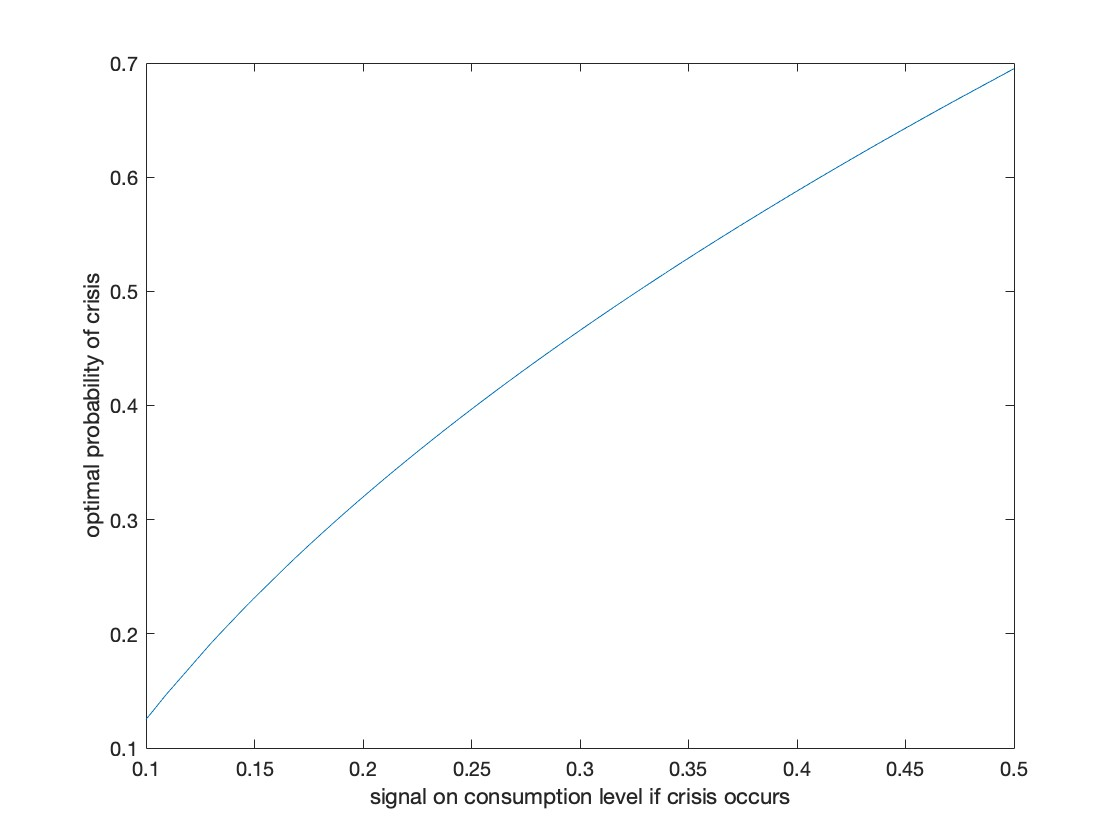
\includegraphics[width=0.8\linewidth]{images/Figure1base} 

}

\caption{Optimal probability of crisis as mapped from the different beliefs of the optimal consumption level}\label{fig:unnamed-chunk-1}
\end{figure}

This model builds on Besley \& Coate (1998)'s model which selects
candidates exogenously and assumes complete information and instead
assumes imperfect information and unique signals that are randomly
provided to each voter.

\hypertarget{voters}{%
\subsection*{Voters}\label{voters}}
\addcontentsline{toc}{subsection}{Voters}

Besley \& Coate (1998) finds that according to the median voter result
and Condorcet Jury theorem, there is one ultimate winning candidate
which is the median voter. According to the median voter theorem, if
preferences are single peaked (which is implied by the uniformly
distributed signals that determine preferences and beliefs about the
probability of crisis) then the median voter will be the winning
candidate in a vote, if we assume voter sincerity (*ref).

Assume democracy

Assume simple majority voting and that each candidate could be running
for public office, thus each voter considers each pairwise comparison
between each individual. Voters are assumed to know that candidates
could only implement their preferred policy, in this context their
individual optimal consumption point and how this maps onto their
optimal probability of crisis. Besley \& Coate (1998) voters voting
decisions are their best response given the rest of voters decisions.
Use the same assumption that candidates cannot credibly commit to any
other policy other than their own policy preference and voters know
this, which is realistic.

\hypertarget{model-set-up-of-sustainable-consumption-in-two-country-economy-with-bargaining}{%
\section{Model set-up of sustainable consumption in two-country economy
with
bargaining}\label{model-set-up-of-sustainable-consumption-in-two-country-economy-with-bargaining}}

(approx 1250 but now 650)

To develop the model set-up further, the impact of another country's
consumption level on the optimal level of consumption is incorporated.
The implications of a two-country model that consider the
interdependence between countries is more realistic, for example in an
IEA, especially considering that global climate change cannot be
achieved by one country acting unilaterally (ref?).

As in the global democracy model set-up, each citizen in each country
receives private signals \(\hat{\underline{c}}_k\) which determine their
optimal level of individual consumption and this maps onto their optimal
probability of crisis. Accordingly, if individuals are signalled to
believe that the climate crisis would not reduce \(c_2\) by much, then a
higher probability of this climate crisis occurring is not worrisome.

Individuals in the global economy are split into two different country
populations after each individual has received their private signals.
Each individual is divided probabilistically into country A and country
B to ensure random splitting. The probability of being assigned to
country A depends on two parameters (\(countryAshare\) and \(bias\)) in
addition to the cumulative density function (\(cdf\)) of each
individual's private signal. For each individual, a number is drawn
between 0 and 1 and if this draw is less than or equal to the
probability of country A, then the individual is assigned to country A.
If not, the individual is assigned to country B.

\[probability_{of}country A = country A share + bias(cdf_{of}signal - country A share)\]

Second, the expected utilities for every possible candidate are computed
under the assumption that each citizen runs for election and promises to
implement their their ideal consumption if elected. Accordingly, each
voter considers any pairwise competition based on the expected utility
they will obtain based on their own belief about \(\tilde{c}\) as formed
due to their private signal \(\hat{\underline{c}}_k\) if the any
candidate implements their promised, preferred policy.

In addition to the fixed parameters discussed in the preceding section,
there are adjustable parameters in the two country case. Variations in
country share A can be implemented by selecting a value between 0 and
0.5, which alters the target fraction of the global democracy population
that will be probabilistically assigned to country A. Variations in bias
can be implemented by selecting a value between 0 and 0.9. This
represents the bias in country A as if the value is higher, then country
A's voters are more likely to receive higher signals and thus are more
likely to believe a higher optimal consumption level and a higher
optimal probability of crisis. To compare the voting outcomes between
different scenarios, three variations of the two-country model are
estimated. Firstly, the 0.1 country A share case in which the size of
two-countries differ dramatically. Secondly, the 50/50 country split
case in which each country is equal in size. Lastly, the 0.9 bias for
country A case in which country A is more likely to contain individuals
who received a higher private signal, and thus have a higher optimal
consumption level and higher optimal probability of crisis.

Next, find the mutual best responses for each country given what the
other country's beliefs based on their private signals are. Each country
votes for the candidate that will yield the best response given how the
other country votes to maximise expected utility. For example, if
country A is biased to consume at a high level, then it would be a best
response for country B to consume at a lower level to reduce the
probability of crisis to be closer to country B's optimal probability of
crisis. The Nash equilibrium in the two-country model is determined
using Matlab's built-in optimisers. In each country, each indiviual has
a best response function and vote for the median candidate, as found in
the median voter theory (ref??), conditional on the other country's
consumption level.

\hypertarget{discussion-and-results}{%
\section{Discussion and results}\label{discussion-and-results}}

(approx 1700 but now 900)

To analyse whether co-operation in the political economy between two
countries is harmful for environmental policies and mitigating climate
crisis, the global democracy model set-up is compared to three
variations of the two-country case. Buchholz \emph{et al} (2005)
compares the isolationist case of one country implementing climate
policies unilaterally against the bargaining case with an IEA
implemented between two countries to analyse the impact of IEAs on
environmental policy. Similarly, this paper compares the global
democracy of one global economy against the Nash equilibrium solution
found in the case of two countries which bargain together according to
an IEA.

Buchholz \emph{et al} (2005) reaches an analytical result in which
voters may be incentivised to vote for less green candidates in order to
improve their own country's bargaining position when there is an IEA,
which implies that unless there is full co-operation, any bargaining
outcome is bad for environmental policy and the probability of a climate
crisis. Besley \& Coate (1998) also suggests that non-co-operation with
other countries may yield a greater expected utility than if
co-operation occurs.

Voters in global economy vote for the median because this maximises
their expected utility.

Are imbalances good or bad???? Unless there is full co-operation, any
bargaining is sub-optimal

\newpage

\begin{figure}[H]

{\centering 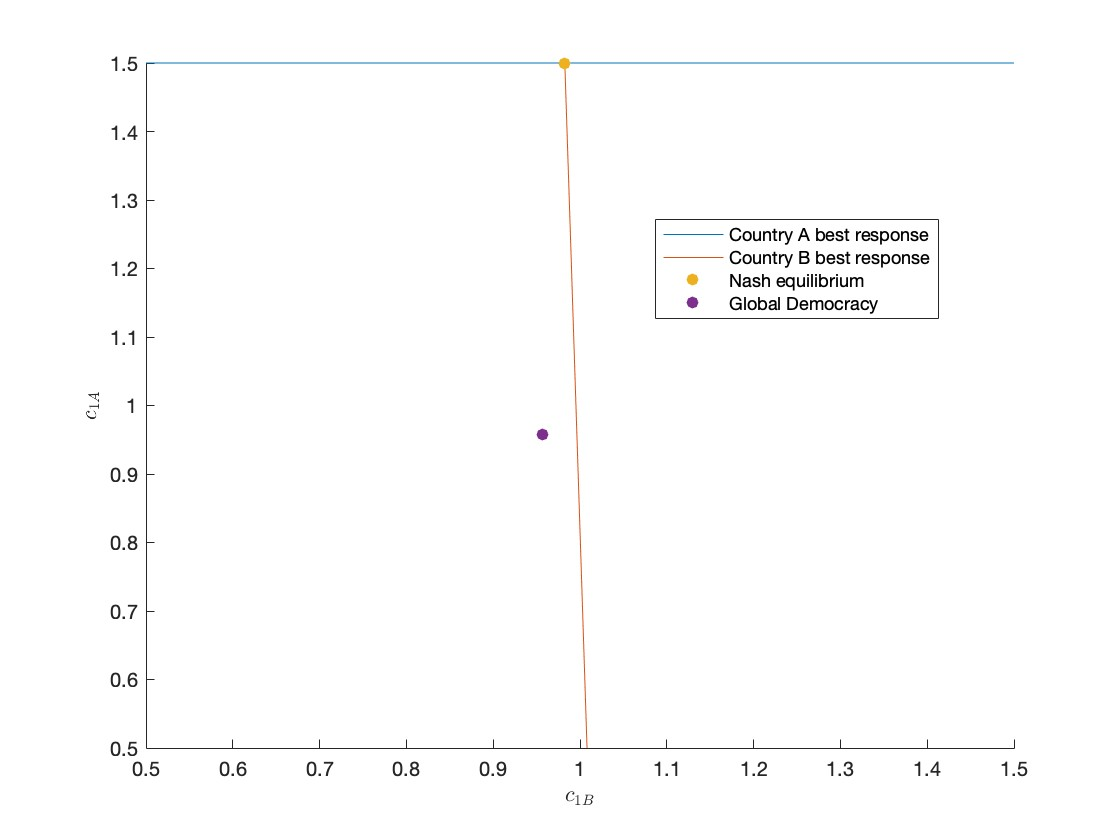
\includegraphics[width=0.45\linewidth]{images/Fig2_0.1Size0Bias} 

}

\caption{Nash equilibrium for 0.1 country A share}\label{fig:unnamed-chunk-2}
\end{figure}

\begin{figure}[H]

{\centering 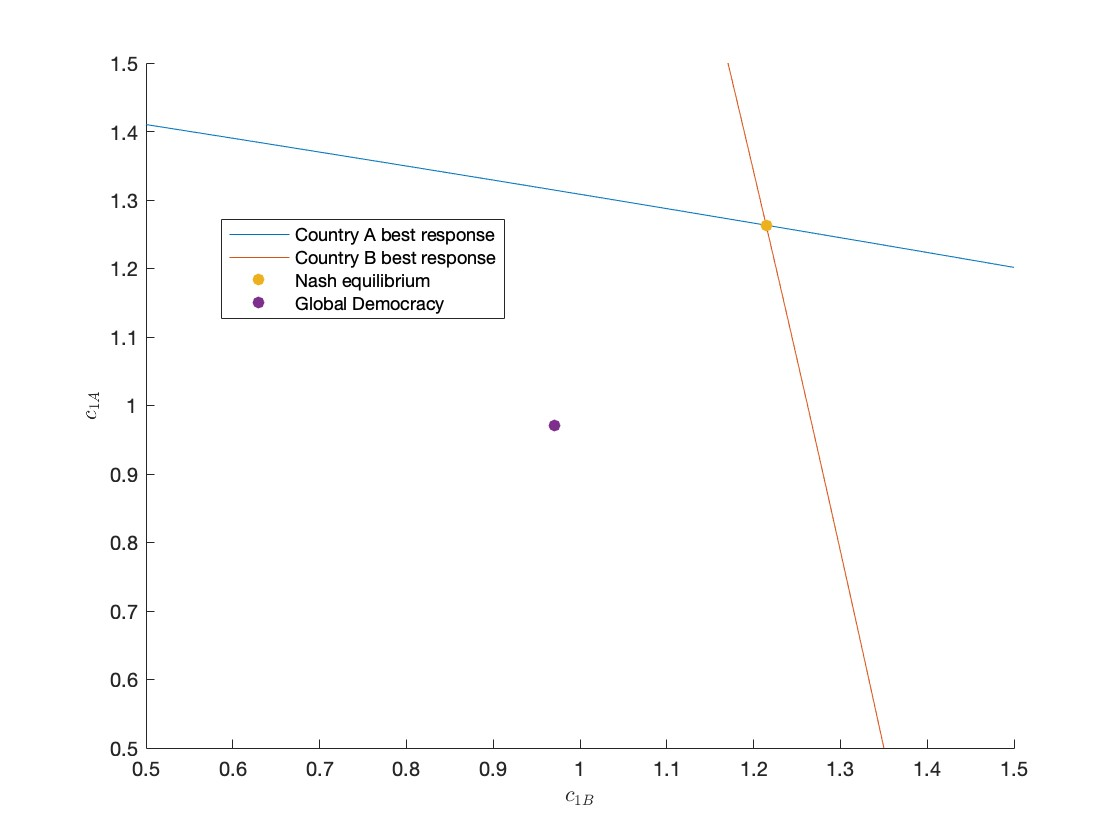
\includegraphics[width=0.45\linewidth]{images/Fig2_0.5Size0Bias} 

}

\caption{Nash equilibrium for 50/50 country split}\label{fig:unnamed-chunk-3}
\end{figure}

\begin{figure}[H]

{\centering 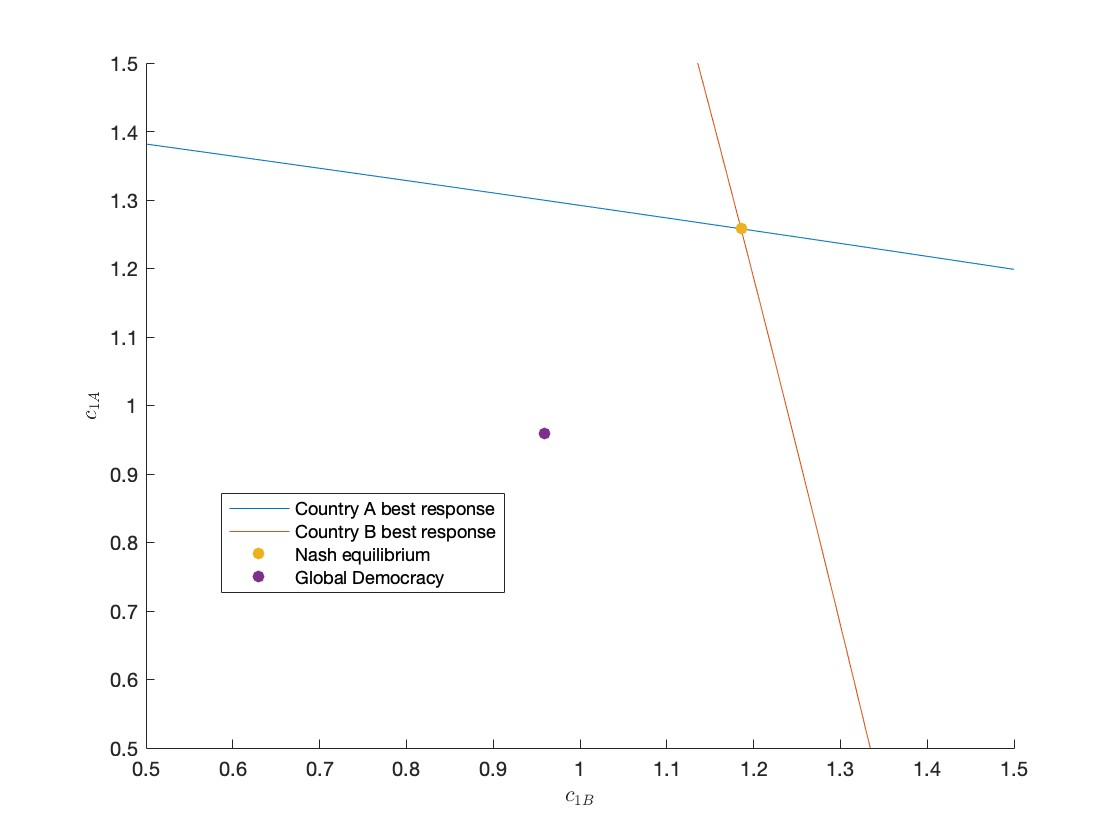
\includegraphics[width=0.45\linewidth]{images/Fig2_0.5Size0.9Bias} 

}

\caption{Nash equilibrium for 0.9 bias for country A}\label{fig:unnamed-chunk-4}
\end{figure}

\hypertarget{country-a-share-0-bias}{%
\subsection*{0.1 Country A share 0 Bias}\label{country-a-share-0-bias}}
\addcontentsline{toc}{subsection}{0.1 Country A share 0 Bias}

In the first variation of the two-country model, the country A share
parameter is set to 0.1, which means that the probabilistic assignment
of an individual being a citizen in country A is smaller. In our
numerical simulation, the result of this is that the population in
country A is 104 and in country B is 896. This demonstrates that the
probabilistic assignment results in a random and imperfect
assignment(??).

\begin{figure}[H]

{\centering 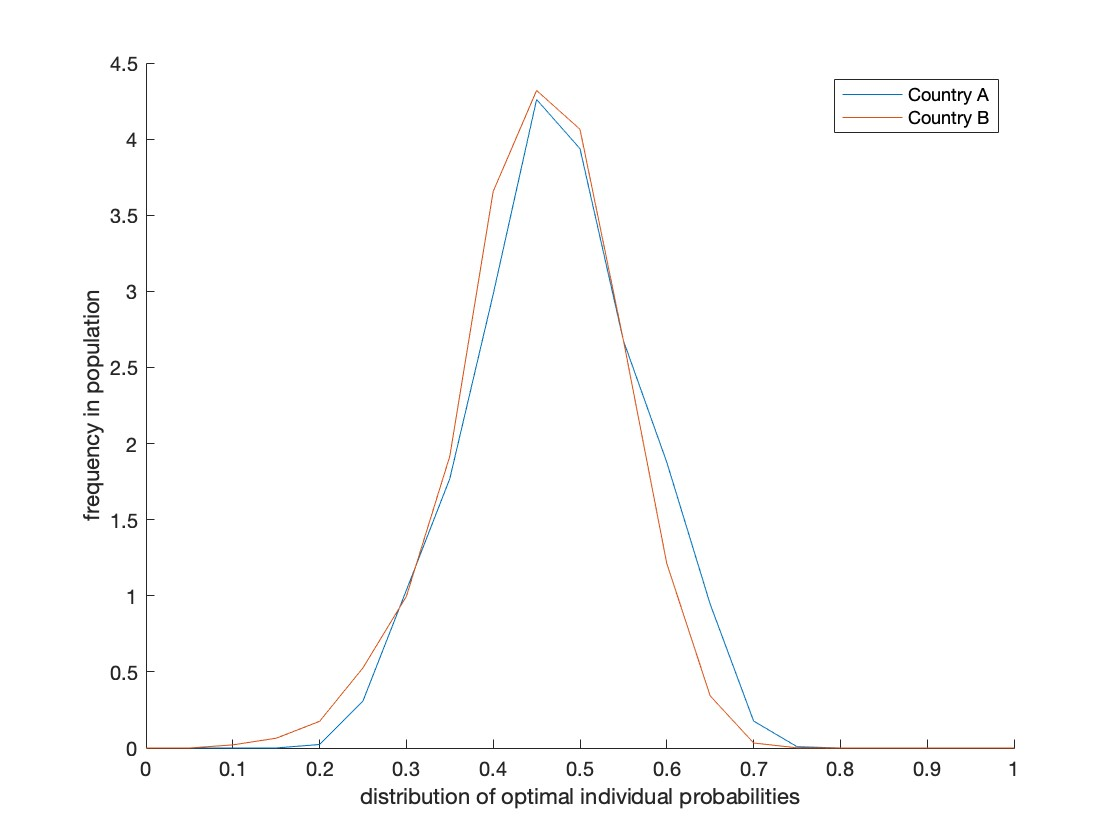
\includegraphics[width=0.8\linewidth]{images/Fig4_0.1Size0Bias} 

}

\caption{0.1 Country A share model: Kernel density function of the distribution of the optimal probabilty of crisis and frequency thereof across individuals in country A and country B}\label{fig:unnamed-chunk-5}
\end{figure}

As in Figure 5.1, when country A has a significantly smaller population
size it is a best response for country A to consume at the highest
threshold \(c_1=c_H=1.5\) that is possible irrespective of the
consumption level that country B chooses. On the other hand, country B's
best response is to consume at a significantly lower level of
approximately \(c_1=1\) irrespective of what country A consumes. Some of
this higher consumption level in country A may be due to the higher
private signals given to country A citizens, as in Figure
(\textgreater\textgreater). In comparison to the global democracy point
plotted on the Figure 5.1, both countries consume more in period 1 which
could only be optimal if both countries' individuals believe that a
higher probability of crisis is optimal. However, this difference in
beliefs is not the case in this model variation because it only differs
from the global democracy in one aspect, which is the country size. Thus
this outcome is slightly less efficient than the global democracy case,
as the probability of crisis in Nash equilibrium is higher, as in Table
1.

\hypertarget{country-a-share-and-0-bias}{%
\subsection*{0.5 Country A share and 0
Bias}\label{country-a-share-and-0-bias}}
\addcontentsline{toc}{subsection}{0.5 Country A share and 0 Bias}

In this model variation, the share of each country's population is
50/50, as the parameter of country A share is set to 0.5. As a result,
the population size in our estimation for country A was 484 and 516 for
country B. This model serves to show how two countries which are of
similar sizes may impact each other's consumption levels. There is no
bias introduced in this model and, as in the previous model variation,
both countries receive signals that are uniformly distributed (Figure
(5.5).

The comparison of Figure 5.2 against 5.1 and the global democracy point
shows that when two countries are similarly sized, each country's best
response is to consume at higher levels. Thus, the Nash equilibrium
point is much higher at \(c_1=1.2134\) for each country. Similar to the
previous model of 0.1 country A share, the beliefs of individuals has
not been adjusted. Figure 5.5 shows that most individuals believe that
approximately 0.52 is the optimal probability of crisis. Therefore, a
higher consumption point as a Nash equilibrium in this model is
sub-optimal and welfare-reducing for both countries.

\begin{figure}[H]

{\centering 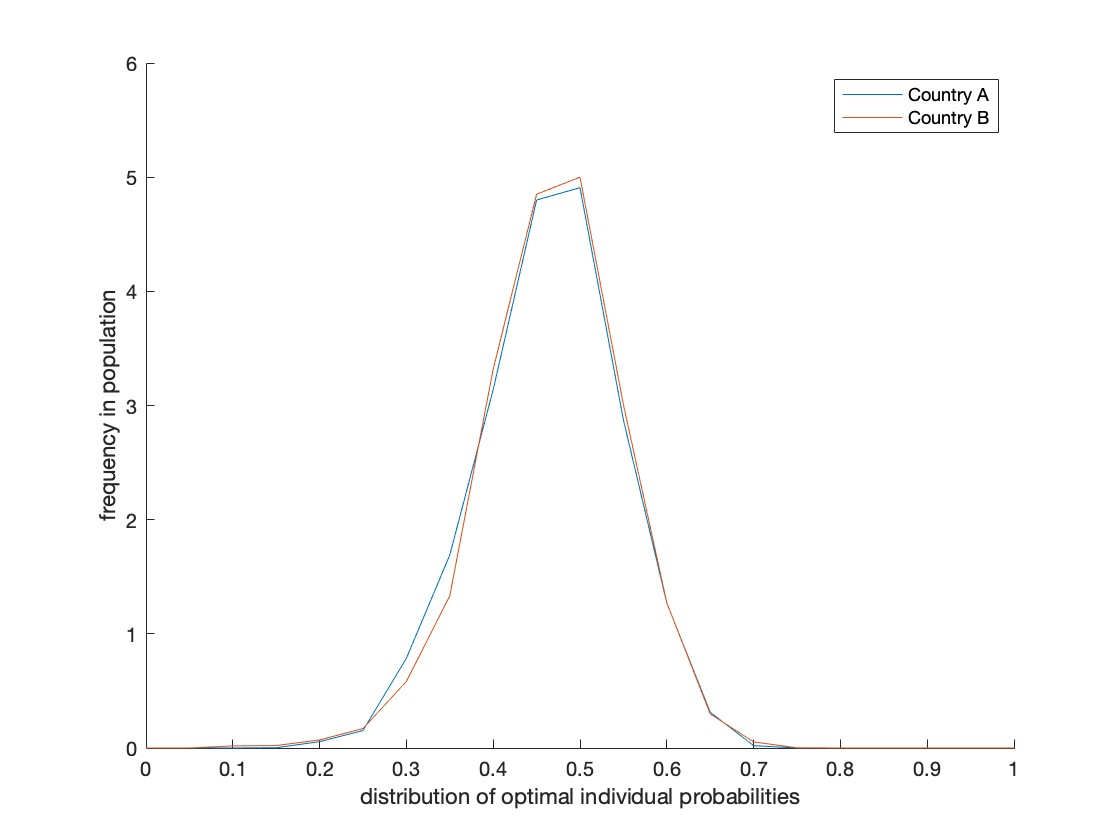
\includegraphics[width=0.8\linewidth]{images/Fig4_0.5Size0Bias} 

}

\caption{50/50 country split model: Kernel density function of the distribution of the optimal probabilty of crisis and frequency thereof across individuals in country A and country B}\label{fig:unnamed-chunk-6}
\end{figure}

\hypertarget{country-a-share-0.9-bias}{%
\subsection*{0.5 Country A share 0.9
Bias}\label{country-a-share-0.9-bias}}
\addcontentsline{toc}{subsection}{0.5 Country A share 0.9 Bias}

In our final variation model, a change in the parameter for bias is
implemented. As aforementioned, a higher bias value means that there is
a higher probability that individuals in country A will receive higher
private signals and believe that a higher consumption level and
probability of crisis is optimal. The population is kept at 50/50, and
is 523 for country A and 477 for country B in this estimation.

Table 1 shows that this final model yields both the highest period one
consumption for country B and the highest probability of crisis.
Therefore, it seems that the worst outcome across the four models
considered is the situation in which two countries are approximately
equal in size but one country receives fundamentally different private
signals about climate change. In Figure 5.3, the Nash equilibrium
consumption point is significantly higher than the global democracy
point.

However, to compare Figure 5.2 and Figure 5.3, the difference in Nash
equilibrium points is not significantly different. Thus it is worse to
go from a large-small country scenario to a two equal sized country
scenario.

The probability of crisis in Nash equilibrium for this model variation
is 0.7234, which is the optimal probability of crisis for less than one
individual in country A and no individuals in country B. Moreover,

\begin{figure}[H]

{\centering 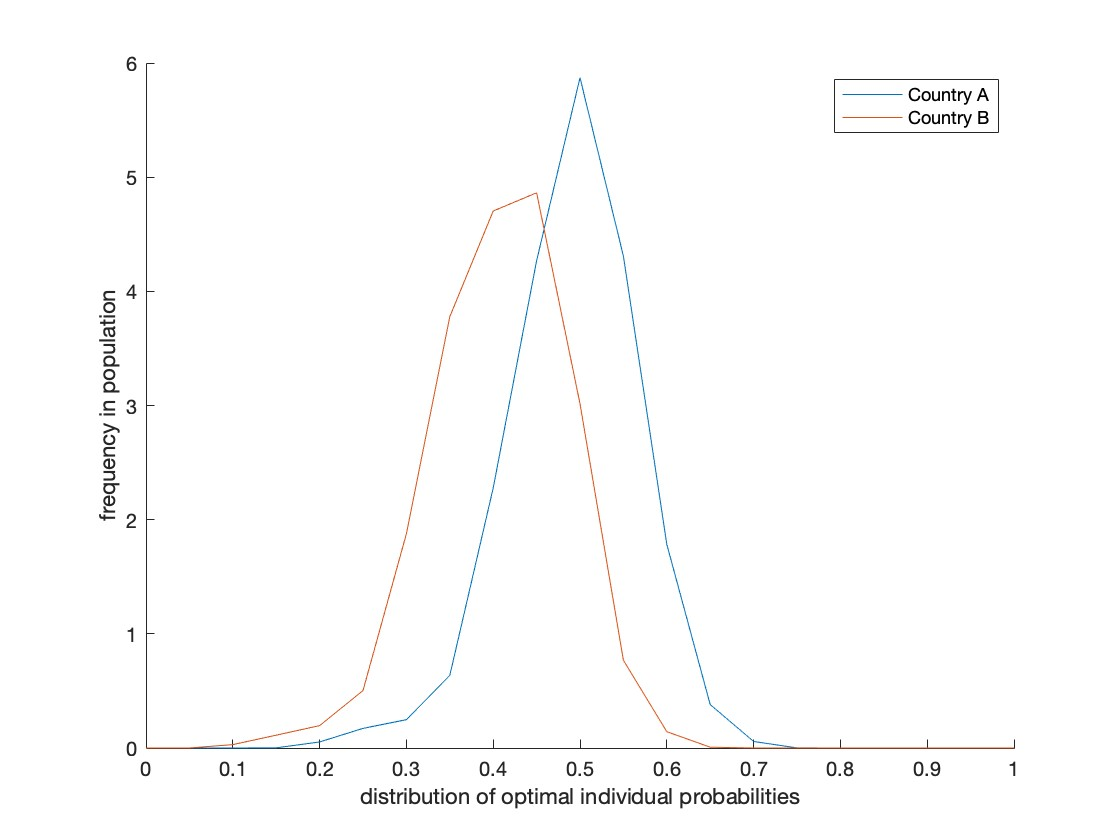
\includegraphics[width=0.8\linewidth]{images/Fig4_0.5Size0.9Bias} 

}

\caption{0.9 Country A bias model: Kernel density function of the distribution of the optimal probabilty of crisis and frequency thereof across individuals in country A and country B}\label{fig:unnamed-chunk-7}
\end{figure}

Kemp (1976) comparative static results

\begin{center}
Table 1: Nash equilibrium values for country B's period one consumption and the probabiility of crisis across four different model variations
\end{center}

\begin{longtable}[]{@{}
  >{\raggedright\arraybackslash}p{(\columnwidth - 6\tabcolsep) * \real{0.2286}}
  >{\centering\arraybackslash}p{(\columnwidth - 6\tabcolsep) * \real{0.2857}}
  >{\centering\arraybackslash}p{(\columnwidth - 6\tabcolsep) * \real{0.2857}}
  >{\centering\arraybackslash}p{(\columnwidth - 6\tabcolsep) * \real{0.2000}}@{}}
\toprule()
\begin{minipage}[b]{\linewidth}\raggedright
\end{minipage} & \begin{minipage}[b]{\linewidth}\centering
Country A period 1 consumption
\end{minipage} & \begin{minipage}[b]{\linewidth}\centering
Country B period 1 consumption
\end{minipage} & \begin{minipage}[b]{\linewidth}\centering
Probability of crisis
\end{minipage} \\
\midrule()
\endhead
Global democracy & 0.9499 & N/A & 0.4499 \\
Two countries 0.1 share & 1.5 & 1.0363 & 0.5363 \\
Two countries 0.5 share & 1.2134 & 1.2134 & 0.7134 \\
Two countries 0.9 bias & 1.2234 & 1.2234 & 0.7234 \\
\bottomrule()
\end{longtable}

\hypertarget{conclusion}{%
\section{Conclusion}\label{conclusion}}

\newpage

\hypertarget{references}{%
\section*{References}\label{references}}
\addcontentsline{toc}{section}{References}

\bibliography{Tex/ref}





\end{document}
